%%%%%%%%%%%%%%%%%%%%%%%%%%
% MSc COM6906 Dissertation Report
%  Manu Kenchappa Junjanna
% University of Sheffield
% 22 March 2017
%%%%%%%%%%%%%%%%%%%%%%%%%%


\documentclass[11pt,oneside]{book}
\usepackage[margin=1.2in]{geometry}
\usepackage{setspace}
\usepackage[toc,page]{appendix}
\usepackage[none]{hyphenat} % turn hyphenation off by default
\usepackage{graphicx}

\begin{document}

\frontmatter

\begin{titlepage}

% You need to edit the details here

\begin{center}

\includegraphics[width=5cm]{images/UOSLogo_Portrait_Violet_RGB.png}\\[2cm]
\linespread{1.2}\huge {\bfseries Project title}\\[2cm]
\linespread{1}
{\Large Manu Kenchappa Junjanna}\\[1cm]
{\large \emph{Supervisor:} Dr Po Yang}\\[1cm]
\large \emph{A report submitted in fulfilment of the requirements}\\ \emph{for the degree of} MSc in Advanced Computer Science\\[0.3cm] 
\textit{in the}\\[0.3cm]
Department of Computer Science\\[2cm]
\today
\end{center}

\end{titlepage}

% -------------------------------------------------------------------
% Declaration
% -------------------------------------------------------------------

\newpage
\chapter*{\Large Declaration}

\setstretch{1.1} % set the line spacing differently if you wish, but this looks good to me. 

All sentences or passages quoted in this report from other people's work have been specifically acknowledged by clear cross-referencing to author, work and page(s). Any illustrations that are not the work of the author of this report have been used with the explicit permission of the originator and are specifically acknowledged. I understand that failure to do this amounts to plagiarism and will be considered grounds for failure in this project and the degree examination as a whole.\\[1cm]

\noindent Name: Manu Kenchappa Junjanna\\[1mm]
\rule[1em]{25em}{0.5pt}

\noindent Signature: Manu KJ\\[1mm]
\rule[1em]{25em}{0.5pt}

\noindent Date: \today \\[1mm]
\rule[1em]{25em}{0.5pt}

% -------------------------------------------------------------------
% Abstract
% -------------------------------------------------------------------

\chapter*{\Large \center Abstract}

Effective pest control has become vital in modern agriculture to maintain crop health and yield.This research project aims to create a novel, user-friendly system that streamlines pest identification and management for farmers by incorporating modern technology. By implementing a secure registration and login system, farmers can easily access the platform and manage their profiles. In order to identify pests accurately and quickly, the system makes use of Machine Learning models that are trained on a large dataset.
Additionally the system provides more details on the pest detected which is backed by a knowledge graph database or a large language model similar to ChatGPT and recommend Pesticides. To enable the purchase of suggested pesticides, a decentralised (peer-to-peer) payment mechanism using blockchain is also included, guaranteeing safe and decentralised transactions.By providing fast, accurate, and feasible pest management solutions, this comprehensive approach not only assists farmers with effective pest control but also encourages sustainable agricultural practices. The integration of modern technology into this system signifies a notable progression in agricultural aid tools, with the potential to enhance farming communities' sustainability and production.


\chapter*{\Large \center Acknowledgement}

I would like to thank Dr. Po Yang, my supervisor, for his continuous support and encouragement during the dissertation process.I extend my thanks to Zhipeng Yuan and Gaoshan Bi for their guidance in writing the paper, and a special thanks to Yang Li from Mutus Tech Ltd for providing APIs related to pest identification, which significantly contributed to the development of the project. Additionally, I want to thank everyone who assisted in testing the usability of my project. 

% -------------------------------------------------------------------
% TOC etc
% -------------------------------------------------------------------

\tableofcontents
\listoffigures
\listoftables

\setstretch{1.1} 

\mainmatter

\chapter{Introduction}

Agriculture began around 12,000 years ago with the transition from nomadic hunter-gatherer cultures to sedentary farming societies. Pests posed a significant obstacle to agriculture as it progressed.Early farmers used crude tactics and natural deterrents to combat a variety of pests.
Today, modern pest control combines traditional methods with innovative technology for example Integrated Pest Management (IPM), discussed in detail in Section 2, has evolved as a sustainable pest management strategy that combines biological, cultural, mechanical, and chemical strategies to manage pest populations while minimising environmental effects. However, the effectiveness of IPM strategies heavily relies on accurate pest identification and the timely application of control measures
(\cite{wikipediacontributors_2019_history}).

Modern technology has made it simpler to access mobile devices and the internet. Using advanced techniques like machine learning and mobile cameras, farmers can quickly identify pests. Large Language Models (LLMs) can provide detailed information about the pests and recommend appropriate pesticides. This project leverages these technologies to create a user-friendly mobile app that identifies pests, provides pesticide recommendations, and integrates blockchain technology for secure and easy purchase of recommended pesticides. This comprehensive solution enhances pest management efficiency, accessibility, and sustainability for farmers.



\section{Aims and Objectives}

This project aims to develop a hybrid application that can run on Android, iOS, and web browsers. The system allows users to upload an image of a pest found on their farm, provides details on how to handle the pest, and recommends pesticides if the pest is hazardous. This comprehensive application uses cutting-edge technology to improve farmers' pest management efficiency and accessibility.

\section{Overview of the Report}

This dissertation is contains 7 chapters. 
\begin{itemize}
    \item Chapter 1 introduces the project background, objectives, and structure of the dissertation.
    \item Chapter 2 explores the literature on the importance of pest control, causes of pests, techniques to control them, comparisons of existing apps, and the tools and technology used in the dissertation.

\end{itemize}
\chapter{Literature Survey}

Lorem ipsum dolor sit amet, consectetuer adipiscing elit. Aenean commodo ligula eget dolor. Aenean massa. Cum sociis natoque penatibus et magnis dis parturient montes, nascetur ridiculus mus. Donec quam felis, ultricies nec, pellentesque eu, pretium quis, sem. Nulla consequat massa quis enim. Donec pede justo, fringilla vel, aliquet nec, vulputate eget, arcu. In enim justo, rhoncus ut, imperdiet a, venenatis vitae, justo. Nullam dictum felis eu pede mollis pretium. Integer tincidunt. Cras dapibus. Vivamus elementum semper nisi. Aenean vulputate eleifend tellus. Aenean leo ligula, porttitor eu, consequat vitae, eleifend ac, enim. \cite{Reference2} Aliquam lorem ante, dapibus in, viverra quis, feugiat a, tellus. Phasellus viverra nulla ut metus varius laoreet. Quisque rutrum. 
\begin{equation}
M = \frac{1}{T}\sum_{t=1}^{T} e(t) / \max_{t}[e(t)]
\end{equation}
Aenean imperdiet. Etiam ultricies nisi vel augue. Curabitur ullamcorper ultricies nisi. Nam eget dui. Etiam rhoncus. Maecenas tempus, tellus eget condimentum rhoncus, sem quam semper libero, sit amet adipiscing sem neque sed ipsum. Nam quam nunc, blandit vel, luctus pulvinar, hendrerit id, lorem. Maecenas nec odio et ante tincidunt tempus. Donec vitae sapien ut libero venenatis faucibus. Nullam quis ante. Etiam sit amet orci eget eros faucibus tincidunt. Duis leo. Sed fringilla mauris sit amet nibh. Donec sodales sagittis magna. Sed consequat, leo eget bibendum sodales, augue velit cursus nunc.

\section{A Section that Contains a Figure}

Lorem ipsum dolor sit amet, consectetuer adipiscing elit. Aenean commodo ligula eget dolor. Aenean massa. Cum sociis natoque penatibus et magnis dis parturient montes, nascetur ridiculus mus. Donec quam felis, ultricies nec, pellentesque eu, pretium quis, sem. Nulla consequat massa quis enim \cite{Reference1}. Donec pede justo, fringilla vel, aliquet nec, vulputate eget, arcu. In enim justo, rhoncus ut, imperdiet a, venenatis vitae, justo. Nullam dictum felis eu pede mollis pretium. Integer tincidunt. Cras dapibus. 
\begin{figure}[ht]
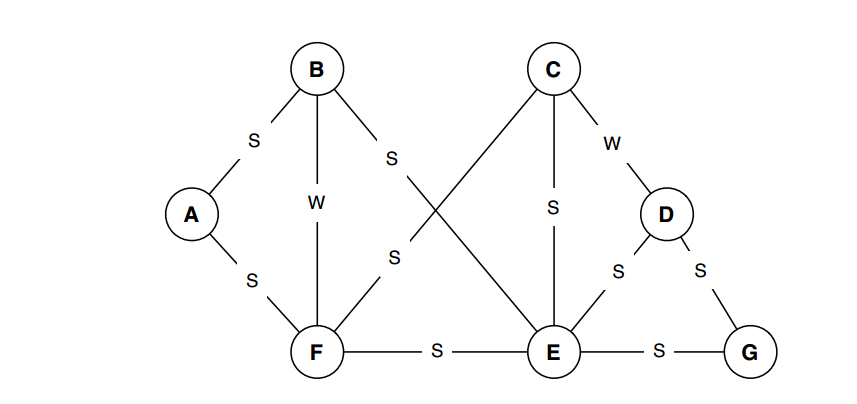
\includegraphics[width=15cm]{figures/figure1.png}
\caption{A simple figure in \LaTeX. Reproduced from http://tinyurl.com/nqtrlj5 with the permission of the copyright owner.}
\label{fig:graph}
\end{figure}
Porttitor eu, consequat vitae, eleifend ac, enim. Aliquam lorem ante, dapibus in, viverra quis, feugiat a, tellus. Phasellus viverra nulla ut metus varius laoreet. Quisque rutrum. Aenean imperdiet. Etiam ultricies nisi vel augue. Curabitur ullamcorper ultricies nisi. Nam eget dui. Etiam rhoncus. Maecenas tempus, tellus eget condimentum rhoncus, sem quam semper libero, sit amet adipiscing sem neque sed ipsum. Nam quam nunc, blandit vel, luctus pulvinar, hendrerit id, lorem. See Figure \ref{fig:graph}. Maecenas nec odio et ante tincidunt tempus. Donec vitae sapien ut libero venenatis faucibus. Nullam quis ante. Etiam sit amet orci eget eros faucibus tincidunt. Duis leo. Sed fringilla mauris sit amet nibh. Donec sodales sagittis magna. Sed consequat, leo eget bibendum sodales, augue velit cursus nunc.

\section{A Section that Contains a Table}

Lorem ipsum dolor sit amet, consectetuer adipiscing elit. Aenean commodo ligula eget dolor. Aenean massa. Cum sociis natoque penatibus et magnis dis parturient montes, nascetur ridiculus mus. Donec quam felis, ultricies nec, pellentesque eu, \cite{Reference3} pretium quis, sem. Nulla consequat massa quis enim. Donec pede justo, fringilla vel, aliquet nec, vulputate eget, arcu. In enim justo, rhoncus ut, imperdiet a, venenatis vitae, justo. Nullam dictum felis eu pede mollis pretium. Integer tincidunt. Cras dapibus. Vivamus elementum semper nisi. Aenean vulputate eleifend tellus. Aenean leo ligula, 

\begin{table}[ht]
\center
\begin{tabular}{cc|c}
A & B & A XOR B\\
\hline
0 & 0 & 0\\
0 & 1 & 1\\
1 & 0 & 1\\
1 & 1 & 0\\
\end{tabular}
\caption{A simple table in \LaTeX.}
\label{tab:xor}
\end{table}

porttitor eu, consequat vitae, eleifend ac, enim. Aliquam lorem ante, dapibus in, viverra quis, feugiat a, tellus. Phasellus viverra nulla ut metus varius laoreet. Quisque rutrum. Aenean imperdiet. Etiam ultricies nisi vel augue. Curabitur ullamcorper ultricies nisi. Nam eget dui. Etiam rhoncus. Maecenas tempus, tellus eget condimentum rhoncus, sem quam semper libero, sit amet adipiscing sem neque sed ipsum. See Table \ref{tab:xor}. Nam quam nunc, blandit vel, luctus pulvinar, hendrerit id, lorem. Maecenas nec odio et ante tincidunt tempus. Donec vitae sapien ut libero venenatis faucibus. Nullam quis ante. Etiam sit amet orci eget eros faucibus tincidunt. Duis leo. Sed fringilla mauris sit amet nibh. Donec sodales sagittis magna. Sed consequat, leo eget bibendum sodales, augue velit cursus nunc.

\section{Summary}

Lorem ipsum dolor sit amet, consectetuer adipiscing elit. Aenean commodo ligula eget dolor. Aenean massa. Cum sociis natoque penatibus et magnis dis parturient montes, nascetur ridiculus mus. Donec quam felis, ultricies nec, pellentesque eu, pretium quis, sem. Nulla consequat massa quis enim. Donec pede justo, fringilla vel, aliquet nec, vulputate eget, arcu. In enim justo, rhoncus ut, imperdiet a, venenatis vitae, justo. Nullam dictum felis eu pede mollis pretium. Integer tincidunt. Cras dapibus. Vivamus elementum semper nisi. Aenean vulputate eleifend tellus. Aenean leo ligula, porttitor eu, consequat vitae, eleifend ac, enim. Aliquam lorem ante, dapibus in, viverra quis, feugiat a, tellus. Phasellus viverra nulla ut metus varius laoreet. Quisque rutrum. Aenean imperdiet. Etiam ultricies nisi vel augue. Curabitur ullamcorper ultricies nisi. Nam eget dui. Etiam rhoncus. Maecenas tempus, tellus eget condimentum rhoncus, sem quam semper libero, sit amet adipiscing sem neque sed ipsum. Nam quam nunc, blandit vel, luctus pulvinar, hendrerit id, lorem. Maecenas nec odio et ante tincidunt tempus. Donec vitae sapien ut libero venenatis faucibus. Nullam quis ante. Etiam sit amet orci eget eros faucibus tincidunt. Duis leo. Sed fringilla mauris sit amet nibh. Donec sodales sagittis magna. Sed consequat, leo eget bibendum sodales, augue velit cursus nunc.

\chapter{Analysis}
This chapter focuses on various types of analyses that need to be conducted before the design and implementation of the application. To begin with, Section 3.1 discusses the project requirements, covering both functional and non-functional aspects.

\section{Project Requirements}

Establishing project requirements is a crucial step in application development, as it outlines the overall functionality of the application and provides clarity to the development process from the user's perspective. Typically, these requirements, which are documented before the development begins, are categorized into functional and non-functional requirements. The remainder of this section will address each of these categories separately.

\subsection{Functional Requirements}
Functional requirements outline the specific behaviors and functionalities that the application must possess to meet the needs of its users. These requirements define what the system should do, detailing the essential features and capabilities that the application must implement to achieve its intended purpose

\begin{table}[H]
    \centering
    \begin{tabular}{|c|>{\centering\arraybackslash}p{0.5\linewidth}|c|c|}
               \hline
        \textbf{No.} & \textbf{Functional Requirements} & \textbf{Priority} & \textbf{Completion} \\
        \hline
        1 & As a user, I can see the introduction of the application. & Mandatory & Completed \\
        \hline
        2 & As a user, I can log in with a username and password. & Mandatory & Completed \\
        \hline
        3 & As a user, I can register with full name, username, email, mobile number, and password. & Mandatory & Completed \\
        \hline
        4 & As a user, I can change the language of the app. & Mandatory & Completed \\
        \hline
    \end{tabular}
    \label{tab:table1}
\end{table}

\begin{table}[H]
    \centering
    \begin{tabular}{|c|>{\centering\arraybackslash}p{0.5\linewidth}|c|c|}
               \hline
5 & As a user, I can log out once logged in. & Mandatory & Completed \\
        \hline
        6 & As a user, I can capture an image to detect the pest. & Mandatory & Completed \\
        \hline
        7 & As a user, I can pick an image that I have already captured for pest detection. & Mandatory & Completed \\
        \hline
        8 & Once the pest is detected, I can see all detected pest names and the pests indicated with bounding boxes. & Mandatory & Completed \\
        \hline
        9 & As a user, I can view details of the detected pests. & Mandatory & Completed \\
        \hline
        10 & As a user, I can add precautions given by the system as a task. & Mandatory & Completed \\
        \hline
        11 & As a user, I can connect and disconnect my Ethereum wallet. & Mandatory & Completed \\
        \hline
        12 & As a user, I can buy pesticides recommended by the system using my Ethereum wallet. & Mandatory & Completed \\
        \hline
        13 & As a user, I can move tasks between the completed and uncompleted sections. & Mandatory & Completed \\
        \hline
        14 & As a user, I can view the transactions of all previous purchases. & Mandatory & Completed \\
        \hline
        \end{tabular}
    \caption{Functional Requirements}
    \label{tab:table1continue}
\end{table}

\subsection{Non-Functional Requirement}
Non-functional requirements are crucial for defining how a system should perform and the constraints it operates under, focusing on aspects like performance, usability, reliability, and security rather than the specific functionalities it provides. Based on your functional requirements, here are some potential non-functional requirements for your application:

\begin{table}[H]
    \centering
    \begin{tabular}{|c|>{\centering\arraybackslash}p{0.5\linewidth}|c|c|} 
    \hline
        \textbf{No.} & \textbf{Non-Functional Requirements} & \textbf{Priority} & \textbf{Completion}\\
             \hline
        1 & The application should handle up to 100 concurrent users without a noticeable decrease in performance or responsiveness. & High & Completed \\
        \hline
        2 & The app should have an intuitive user interface that allows new users to understand the system within 10 minutes of use. & Mandatory & Completed \\
        \hline
        3 & Users should be able to seamlessly switch between supported languages without disruption. & Mandatory & Completed \\
        \hline
    \end{tabular}
    \label{tab:table2}
\end{table}

\begin{table}[H]
    \centering
    \begin{tabular}{|c|>{\centering\arraybackslash}p{0.5\linewidth}|c|c|} 
    \hline
        \textbf{No.} & \textbf{Non-Functional Requirements} & \textbf{Priority} & \textbf{Completion}\\
         \hline
        % \hline
        %  1 & The system should analyze and provide pest detection results within 5 seconds of capturing or uploading an image. & High & Pending \\
       
        4 & The application should handle errors gracefully and provide meaningful error messages without crashing. & Mandatory & Completed \\
        \hline
        5 & All sensitive user data must be encrypted in transit and at rest using industry-standard encryption methods. & Mandatory & Pending \\
        \hline
        6 & The application should implement Token-Based Authentication  for user accounts. & High & Completed \\
        \hline
        7 & The application should be compatible with major mobile platforms in both IOS and Android & Mandatory & Completed \\
        \hline
        8 & The codebase should be well-documented and follow best practices for maintainability. & High & Completed \\
        \hline
        9 & The system should include robust logging and monitoring mechanisms to track errors and performance issues. & Mandatory & Pending \\
        \hline
        10 & The application should include validation checks to ensure data accuracy and consistency. & Mandatory & Completed \\
        \hline
        % 11 & Regular backups should be performed, with tested recovery procedures to protect against data loss. & High & Not Started \\
        % \hline
        11 & The application must adhere to relevant regulations and standards, including data protection laws such as GDPR. & Mandatory & Completed \\
        \hline
        12 & The application should support localization features to adapt to various regional settings, such as date formats and currencies. & High & Completed \\
        \hline
        13 & The system should be capable of scaling horizontally to accommodate increasing user numbers or data volumes. & High & Pending \\
        \hline
    \end{tabular}
    \caption{Non Functional Requirement}
    \label{tab:table2Continue}
\end{table}

    
\section{Blockchain Payment vs Centralized Payment Methods}

Blockchain is a distributed ledger technology that ensures transparency, security, and immutability of transactions, In this project blockchain is used as a payment method for purchasing pesticides. This below table explains why a blockchain payment approach is necessary and compares it to traditional centralized payment methods. \cite{centralised_vs_decentralised}.


\begin{table}[H]
    \centering
    \begin{tabular}{|>{\centering\arraybackslash}p{0.12\linewidth}|p{0.45\linewidth}|p{0.45\linewidth}|} \hline 
    \textbf{Aspect} & \textbf{Centralized   } & \textbf{Blockchain Systems}\\
        \hline
        Structure and Operation  
        & 
        Centralised system works through a network of banks and financial institutions with a central authority, who manages and oversees all the transactions
        &
        Blockchain works without a central authority. Instead, a distributed public ledger is used to record and verify transactions by the network participants using a consensus mechanism.
        \\
        \hline
        Risks 
        & 
        One of the major risks in centralized payment systems is that they are completely dependent on a single entity, and if that entity fails, the whole system goes down. Additionally, banks might temporarily lack the liquidity to settle transactions.
        & 
        While blockchain technology is secure, its decentralized nature can also pose risks, such as a 51\% attack, where a single entity gains control of the majority of the network's mining power and has the ability to rewrite the source of truth within the network.
        \\
        \hline
        Acceptance 
        & 
        Traditional payment systems, such as banks, have a long history and have been widely accepted and trusted by users, leading to broad acceptance.
        & 
        Blockchain technology has gained popularity in recent years, but the majority of population has not yet fully accepted it.
        \\
        \hline
        Law and Regulation  
        & 
        Centralized systems are highly regulated and monitored by governmental and financial bodies to ensure stability and compliance with financial laws.
        &
        One of the fundamental features of blockchain systems is the absence of a central governing body. This inherently reduces the ability of any single entity or government to directly control or regulate the system.
        \\
        \hline
        Privacy 
        &
       Mostly managed by a single central entity, which can lead to potential data exposure and misuse.
        & 
        In blockchain, privacy is enhanced by distributing control across multiple participants. 
        \\
        \hline
    \end{tabular}
    \caption{Comparison between Blockchain Payment vs Centralized Payment Method}
    \label{tab:centralised_and_blockchain}
\end{table}

For the purpose of purchasing pesticides in this project, using blockchain seems to be a better approach than traditional centralized payment methods, mainly because of the privacy it offers to users. Blockchain ensures that no single entity has the power to misuse user data. Additionally, the distributed ledger eliminates the need for a centralized entity, which not only enhances security but also minimizes the risks associated with centralized failures and liquidity issues. 

\section{Ethics Considerations}
In this section, let's discuss the ethical issues related to the project, including topics such as intellectual property and data privacy.
\begin{itemize}
    \item Intellectual property: This project is more than just a study of software engineering; it additionally incorporates significant findings from agricultural research, mainly in the areas of pest management and environmental impact.Section 2 contains a comprehensive and thorough study on pest identification, the causes of infestations, and IPM ( Integrated Pest Management).All content (e.g., phrases, figures, etc.) from other researchers' papers utilised in this project has been officially authorised by the copyright holders and is cited immediately following quotes.Furthermore, the app implementation and UI/UX ( User Interface and User Experience) are entirely original, having been created after substantial background study and literature evaluation.
    \item Data Privacy and Security: The application collects and processes sensitive user data, including usernames, email addresses, phone numbers, and images of pests uploaded for detection. All of this data is passed to APIs provided by Mutus Ltd., which stores the data and is obligated to adhere to strict data protection regulations and privacy standards.
    As discussed in Section 3.2, one of the main reasons for selecting a blockchain payment system is to avoid the collection of user payment details, thereby enhancing privacy and security
    \item Environmental Impact and Accountability: The application recommends pesticides based on the detected pest, but the use of pesticides can cause environmental problems. As a precaution, the app first provides step by step guidance on how to handle the pest, and only recommends pesticides as a last resort. Overuse of chemical pesticides can damage non-target species, contribute to pesticide resistance, and worsen environmental health. To further reduce these risks, the application prioritises on Integrated Pest Management (IPM) tactics and provide information on sustainable agricultural practices, encouraging users to choose more environmentally friendly options. 
\end{itemize}

\section{Testing Analysis}
The testing phase is critical to  ensure the reliability, functionality, and user satisfaction of the pest management application. Since the project involves advanced technologies like AI for pest detection, blockchain for secure transactions, and the implementation of cross-platform mobile development frameworks like Flutter, it is critical that each component is extensively tested to ensure smooth integration and strong functioning. Comprehensive testing will help in identifying and resolving possible issues, ensuring the final product meets the highest standards of quality and effectiveness before deployment. This section explores the importance of automation, the testing strategies commonly employed in Flutter, and the tools available to developers \cite{testing_analysis}

\subsection{Importance of Automated Testing}
Automated testing is critical for ensuring application quality as they get increasingly complex. It ensures that new additions and upgrades do not disrupt current functioning. Automated testing is an essential component of the development process in the fast-paced IT business, where speedy and uniform testing is required. It also supports Continuous Integration and Continuous Delivery (CI/CD) pipelines, enabling rapid releases without compromising on quality.

\subsection{Testing Pyramid in Flutter}
The testing pyramid is a widely adopted framework in software testing. In Flutter, this pyramid is composed of:
\begin{figure}[ht]
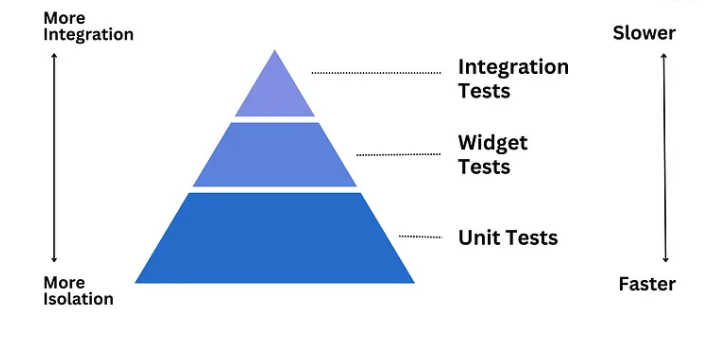
\includegraphics[width=15cm]{myReport/figures/test_pyramid.png}
\caption{Testing Pyramid (Akanksha Gupta, TestVagrant Tech, 2023)}
\end{figure}

\begin{itemize}
    \item Unit Testing: Unit Testing is a primary software testing strategy used in development. It focuses on testing specific components or sections of the application to ensure they perform as intended. By breaking the program down into discrete, testable sections such as individual utility functions or widgets we can verify that each unit functions correctly in isolation
    \item Widget Testing: This includes testing individual widgets to ensure they work properly inside the UI. It is a step up from unit testing, focusing on components rather than the entire system.
    \item Integration Testing: Also known as end-to-end testing, this replicates user interactions inside an application and evaluates the complete application flow, ensuring that all components function together smoothly. 
\end{itemize}


\subsection{Tools for Automation Testing}
\subsubsection{Flutter Integration Test Package}
\begin{itemize}
    \item This package is part of the Flutter SDK and has been designed specifically for end-to-end integration testing in Flutter apps.
    \item It enables developers to run unit, widget, and integration tests, guaranteeing thorough testing across all layers of the application.
\end{itemize}
\subsubsection{Firebase Test Lab}
\begin{itemize}
    \item A cloud-based app testing infrastructure that integrates with Flutter.
    \item Supports running tests across a variety of physical and virtual devices hosted by Google, providing detailed logs, crash reports, and performance data.
\end{itemize}
\subsubsection{CodeMagic}
\begin{itemize}
    \item A CI/CD tool tailored for Flutter apps.
    \item It integrates well with Flutter projects, automating the build, testing, and deployment processes, thus speeding up development and release cycles.
\end{itemize}
\subsubsection{Appium}
\begin{itemize}
    \item A widely-used open-source tool for mobile automation testing.
    \item Although it works on cross platforms, its integration with Flutter is restricted because it does not support all Flutter widgets. It is recommended that you undertake a proof-of-concept to assess its usefulness for certain Flutter applications.
\end{itemize}
.

\chapter{Planning}

\section{Risk Analysis}

Lorem ipsum dolor sit amet, consectetuer adipiscing elit. Aenean commodo ligula eget dolor. Aenean massa. Cum sociis natoque penatibus et magnis dis parturient montes, nascetur ridiculus mus. Donec quam felis, ultricies nec, pellentesque eu, pretium quis, sem. Nulla consequat massa quis enim. Donec pede justo, fringilla vel, aliquet nec, vulputate eget, arcu. In enim justo, rhoncus ut, imperdiet a, venenatis vitae, justo. Nullam dictum felis eu pede mollis pretium. Integer tincidunt. Cras dapibus. Vivamus elementum semper nisi. Aenean vulputate eleifend tellus. Aenean leo ligula, porttitor eu, consequat vitae, eleifend ac, enim. Aliquam lorem ante, dapibus in, viverra quis, feugiat a, tellus. Phasellus viverra nulla ut metus varius laoreet. Quisque rutrum. Aenean imperdiet. Etiam ultricies nisi vel augue. Curabitur ullamcorper ultricies nisi. Nam eget dui. Etiam rhoncus. Maecenas tempus, tellus eget condimentum rhoncus, sem quam semper libero, sit amet adipiscing sem neque sed ipsum. Nam quam nunc, blandit vel, luctus pulvinar, hendrerit id, lorem. Maecenas nec odio et ante tincidunt tempus. Donec vitae sapien ut libero venenatis faucibus. Nullam quis ante. Etiam sit amet orci eget eros faucibus tincidunt. Duis leo. Sed fringilla mauris sit amet nibh. Donec sodales sagittis magna. Sed consequat, leo eget bibendum sodales, augue velit cursus nunc.

\section{Project Plan}

Lorem ipsum dolor sit amet, consectetuer adipiscing elit. Aenean commodo ligula eget dolor. Aenean massa. Cum sociis natoque penatibus et magnis dis parturient montes, nascetur ridiculus mus. Donec quam felis, ultricies nec, pellentesque eu, pretium quis, sem. Nulla consequat massa quis enim. Donec pede justo, fringilla vel, aliquet nec, vulputate eget, arcu. In enim justo, rhoncus ut, imperdiet a, venenatis vitae, justo. Nullam dictum felis eu pede mollis pretium. Integer tincidunt. Cras dapibus. Vivamus elementum semper nisi. Aenean vulputate eleifend tellus. Aenean leo ligula, porttitor eu, consequat vitae, eleifend ac, enim. Aliquam lorem ante, dapibus in, viverra quis, feugiat a, tellus. Phasellus viverra nulla ut metus varius laoreet. Quisque rutrum. Aenean imperdiet. Etiam ultricies nisi vel augue. Curabitur ullamcorper ultricies nisi. Nam eget dui. Etiam rhoncus. Maecenas tempus, tellus eget condimentum rhoncus, sem quam semper libero, sit amet adipiscing sem neque sed ipsum. Nam quam nunc, blandit vel, luctus pulvinar, hendrerit id, lorem. Maecenas nec odio et ante tincidunt tempus. Donec vitae sapien ut libero venenatis faucibus. Nullam quis ante. Etiam sit amet orci eget eros faucibus tincidunt. Duis leo. Sed fringilla mauris sit amet nibh. Donec sodales sagittis magna. Sed consequat, leo eget bibendum sodales, augue velit cursus nunc.

\section{Another Section if You Need It}

Lorem ipsum dolor sit amet, consectetuer adipiscing elit. Aenean commodo ligula eget dolor. Aenean massa. Cum sociis natoque penatibus et magnis dis parturient montes, nascetur ridiculus mus. Donec quam felis, ultricies nec, pellentesque eu, pretium quis, sem. Nulla consequat massa quis enim. Donec pede justo, fringilla vel, aliquet nec, vulputate eget, arcu. In enim justo, rhoncus ut, imperdiet a, venenatis vitae, justo. Nullam dictum felis eu pede mollis pretium. Integer tincidunt. Cras dapibus. Vivamus elementum semper nisi. Aenean vulputate eleifend tellus. Aenean leo ligula, porttitor eu, consequat vitae, eleifend ac, enim. Aliquam lorem ante, dapibus in, viverra quis, feugiat a, tellus. Phasellus viverra nulla ut metus varius laoreet. Quisque rutrum. Aenean imperdiet. Etiam ultricies nisi vel augue. Curabitur ullamcorper ultricies nisi. Nam eget dui. Etiam rhoncus. Maecenas tempus, tellus eget condimentum rhoncus, sem quam semper libero, sit amet adipiscing sem neque sed ipsum. Nam quam nunc, blandit vel, luctus pulvinar, hendrerit id, lorem. Maecenas nec odio et ante tincidunt tempus. Donec vitae sapien ut libero venenatis faucibus. Nullam quis ante. Etiam sit amet orci eget eros faucibus tincidunt. Duis leo. Sed fringilla mauris sit amet nibh. Donec sodales sagittis magna. Sed consequat, leo eget bibendum sodales, augue velit cursus nunc.

\chapter{Conclusions}

Lorem ipsum dolor sit amet, consectetuer adipiscing elit. Aenean commodo ligula eget dolor. Aenean massa. Cum sociis natoque penatibus et magnis dis parturient montes, nascetur ridiculus mus. Donec quam felis, ultricies nec, pellentesque eu, pretium quis, sem. Nulla consequat massa quis enim. Donec pede justo, fringilla vel, aliquet nec, vulputate eget, arcu. In enim justo, rhoncus ut, imperdiet a, venenatis vitae, justo. Nullam dictum felis eu pede mollis pretium. Integer tincidunt. Cras dapibus. Vivamus elementum semper nisi. Aenean vulputate eleifend tellus. Aenean leo ligula, porttitor eu, consequat vitae, eleifend ac, enim. Aliquam lorem ante, dapibus in, viverra quis, feugiat a, tellus. Phasellus viverra nulla ut metus varius laoreet. Quisque rutrum. Aenean imperdiet. Etiam ultricies nisi vel augue. Curabitur ullamcorper ultricies nisi. Nam eget dui. Etiam rhoncus. Maecenas tempus, tellus eget condimentum rhoncus, sem quam semper libero, sit amet adipiscing sem neque sed ipsum. Nam quam nunc, blandit vel, luctus pulvinar, hendrerit id, lorem. Maecenas nec odio et ante tincidunt tempus. Donec vitae sapien ut libero venenatis faucibus. Nullam quis ante. Etiam sit amet orci eget eros faucibus tincidunt. Duis leo. Sed fringilla mauris sit amet nibh. Donec sodales sagittis magna. Sed consequat, leo eget bibendum sodales, augue velit cursus nunc.


\bibliographystyle{acm} 
\bibliography{mybibliography} 

\begin{appendices}
\chapter{An Appendix of Some Kind}

Lorem ipsum dolor sit amet, consectetuer adipiscing elit. Aenean commodo ligula eget dolor. Aenean massa. Cum sociis natoque penatibus et magnis dis parturient montes, nascetur ridiculus mus. Donec quam felis, ultricies nec, pellentesque eu, pretium quis, sem. Nulla consequat massa quis enim. Donec pede justo, fringilla vel, aliquet nec, vulputate eget, arcu. In enim justo, rhoncus ut, imperdiet a, venenatis vitae, justo. Nullam dictum felis eu pede mollis pretium. Integer tincidunt. Cras dapibus. Vivamus elementum semper nisi. Aenean vulputate eleifend tellus. Aenean leo ligula, porttitor eu, consequat vitae, eleifend ac, enim. Aliquam lorem ante, dapibus in, viverra quis, feugiat a, tellus. Phasellus viverra nulla ut metus varius laoreet. Quisque rutrum. Aenean imperdiet. Etiam ultricies nisi vel augue. Curabitur ullamcorper ultricies nisi. Nam eget dui. Etiam rhoncus. Maecenas tempus, tellus eget condimentum rhoncus, sem quam semper libero, sit amet adipiscing sem neque sed ipsum. Nam quam nunc, blandit vel, luctus pulvinar, hendrerit id, lorem. Maecenas nec odio et ante tincidunt tempus. Donec vitae sapien ut libero venenatis faucibus. Nullam quis ante. Etiam sit amet orci eget eros faucibus tincidunt. Duis leo. Sed fringilla mauris sit amet nibh. Donec sodales sagittis magna. Sed consequat, leo eget bibendum sodales, augue velit cursus nunc.

\chapter{Another Appendix}

Lorem ipsum dolor sit amet, consectetuer adipiscing elit. Aenean commodo ligula eget dolor. Aenean massa. Cum sociis natoque penatibus et magnis dis parturient montes, nascetur ridiculus mus. Donec quam felis, ultricies nec, pellentesque eu, pretium quis, sem. Nulla consequat massa quis enim. Donec pede justo, fringilla vel, aliquet nec, vulputate eget, arcu. In enim justo, rhoncus ut, imperdiet a, venenatis vitae, justo. Nullam dictum felis eu pede mollis pretium. Integer tincidunt. Cras dapibus. Vivamus elementum semper nisi. Aenean vulputate eleifend tellus. Aenean leo ligula, porttitor eu, consequat vitae, eleifend ac, enim. Aliquam lorem ante, dapibus in, viverra quis, feugiat a, tellus. Phasellus viverra nulla ut metus varius laoreet. Quisque rutrum. Aenean imperdiet. Etiam ultricies nisi vel augue. Curabitur ullamcorper ultricies nisi. Nam eget dui. Etiam rhoncus. Maecenas tempus, tellus eget condimentum rhoncus, sem quam semper libero, sit amet adipiscing sem neque sed ipsum. Nam quam nunc, blandit vel, luctus pulvinar, hendrerit id, lorem. Maecenas nec odio et ante tincidunt tempus. Donec vitae sapien ut libero venenatis faucibus. Nullam quis ante. Etiam sit amet orci eget eros faucibus tincidunt. Duis leo. Sed fringilla mauris sit amet nibh. Donec sodales sagittis magna. Sed consequat, leo eget bibendum sodales, augue velit cursus nunc.

\end{appendices}

\end{document}
